\documentclass{article}
\usepackage{graphicx} % Required for inserting images
\usepackage[T1,T2A]{fontenc}
\usepackage[utf8]{inputenc}
\usepackage[russian]{babel}
\usepackage{hyperref}

\usepackage{geometry} % Простой способ задавать поля
\geometry{top=20mm}
\geometry{bottom=25mm}
\geometry{left=30mm}
\geometry{right=10mm}

\usepackage{setspace} % Интерлиньяж
\setstretch{1.1}

\newcommand{\coursename}{Causal Inference: прозрение и практика}

\title{
    \textbf{\coursename}\\
    Лекция 1.
    Основные понятия Causal Inference
    }
\author{Юрашку Иван Вячеславович}
\date{\today}

\begin{document}

    % \begin{center}
    %     \textbf
    % \end{center}

    \maketitle

    \section*{Что такое Causal Inference.}

        В современном мире Data Science играет ключевую роль в анализе и использовании данных. Мы живем в эпоху, где информация - это золото, а умение извлекать из нее ценные знания - наша сила. Однако часто понятие Data Science ограничивается лишь алгоритмами машинного обучения или даже искусственным интеллектом, умаляя другие важные аспекты этой дисциплины.

        Вот где начинается история о сближении двух мощных инструментов: эконометрики и Machine Learning. В разных эпохах они казались как бы двумя противоположными полярностями в анализе данных. Машинное обучение стремилось к высокой точности прогнозов, зачастую уступая интерпретируемости моделей. С другой стороны, эконометрика ставила акцент на интерпретируемость, понимание причинно-следственных связей, иногда уходя в тень из-за ограниченности моделей.

        Однако со временем стало понятно, что для полного понимания данных нам нужно объединить эти подходы. И здесь на сцену выходит Causal Inference, или причинно-следственная связь. Этот инструмент помогает нам разгадывать причины за явлениями, объединяя преимущества как машинного обучения, так и эконометрики. Так, Judea Pearl в \href{https://www.degruyter.com/document/doi/10.1515/jci-2021-0006/html}{своей статье} 2021 года подчеркивает важность CI как ключевого элемента для достижения баланса между эмпирическим и интерпретируемым.

        \begin{figure}[h]
            \centering
            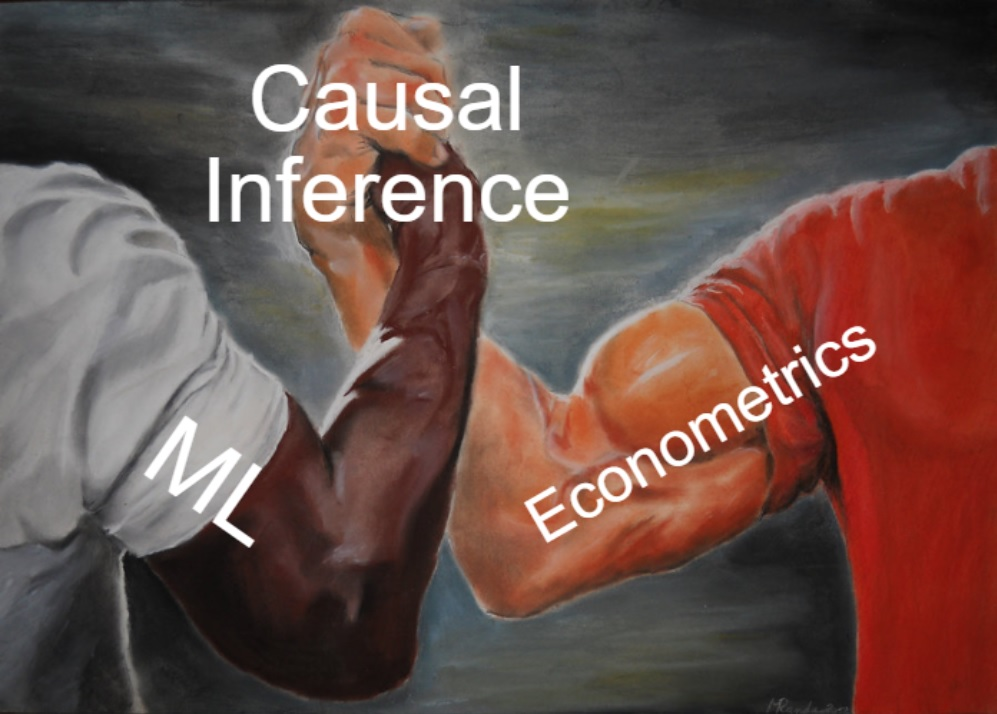
\includegraphics[width=0.7\linewidth]{imgs/epic_CI.jpg}
            % \caption{meme}
            \label{fig:mpr}
        \end{figure}

        \newpage

        Погружение в мир причинно-следственной связи и машинного обучения не только расширит ваш кругозор, но и даст вам ключ к разгадке сложных и важных вопросов, стоящих перед современным обществом.

        Допустим, вы владеете интернет-магазином и хотите понять, какие факторы влияют на продажи. С помощью методов причинно-следственной связи вы сможете определить, какие из ваших маркетинговых кампаний действительно приносят наибольший доход, и направить свои усилия и ресурсы в нужное русло.

        Еще один пример - медицинская сфера. С помощью анализа причинно-следственных связей можно выявить, какие лечебные методы наиболее эффективны для конкретного заболевания, что позволит разрабатывать более точные и эффективные методики лечения.

        Этот курс - не просто набор теории, он предлагает вам практические инструменты для анализа данных и принятия обоснованных решений. С его помощью вы сможете выйти за рамки обычных аналитических методов и раскрыть потенциал данных, лежащих у вас под рукой. Полученные знания не только помогут читателю в работе, но и дадут возможность вносить реальные изменения в мир вокруг нас.

    \section*{И все же Causal Inference - это не ML}
        Машинное обучение в настоящее время успешно решает задачи прогнозирования. Как подчеркивают Ajay Agrawal, Joshua Gans и Avi Goldfarb в книге "Prediction Machines":

        \begin{quote}
            "Новая волна искусственного интеллекта на самом деле приносит нам не интеллект, а важный компонент интеллекта - прогнозирование".
        \end{quote}

        С машинным обучением мы можем совершать самые разнообразные и впечатляющие вещи. Главное требование заключается в том, чтобы сформулировать наши задачи как задачи прогнозирования. Хотите перевести текст с английского на португальский? Тогда создайте модель машинного обучения, которая предсказывает португальские предложения по английским. Хотите распознавать лица? Тогда разработайте модель машинного обучения, которая определяет наличие лица в определенной области изображения. Хотите создать автомобиль с автоматическим управлением? Тогда создайте модель машинного обучения, которая предсказывает направление поворота руля, а также давление на тормоза и акселератор при предоставлении изображений и данных с сенсоров, полученных из окружающей среды автомобиля.


        Однако ML - не панацея. Он может производить чудеса в рамках строгих условий, но при этом может потерпеть крах, если данные немного отличаются от того, что модель привыкла видеть.


        Машинное обучение известно своей неспособностью решать проблемы обратной причинности. Оно требует ответа на вопросы типа "а что, если"{}, которые экономисты называют контрфактуальными. Как отмечается в "Prediction Machines"{}, ML не справляется с такими задачами. Оно может предсказывать на основе данных, но не может оценить воздействие изменений. В качестве примера из книги "Prediction Machines":

        \begin{quote}
            "Во многих отраслях низкая цена ассоциируется с низкими продажами. Например, в гостиничной индустрии цены низки вне туристического сезона, а в период пикового спроса цены высоки и гостиницы полностью заполнены. Исходя из этих данных, наивное предположение может подсказать, что повышение цены приведет к увеличению числа проданных номеров".
        \end{quote}

        По сути, ответ на вопросы о причинности является более сложной задачей, чем многие могут подумать. Это то, чему посвящен курс "\coursename". В нем мы исследуем, как использовать данные для изучения причинно-следственных связей и оценки воздействия вмешательств на результаты. Поехали!

    \section*{"Correlation is not causation"}



    % \section*{В одной далекой-далекой школе.}

    %     В 2020 году пандемия коронавируса заставила бизнес адаптироваться к социальному дистанцированию. Службы доставки стали широко распространенными, и крупные корпорации перешли на стратегию удаленной работы. С образованием дела обстояли так же. Многие начали свой собственный онлайн-репозиторий уроков.

    %     Через четыре месяца кризиса многие задались вопросом, можно ли сохранить внедренные изменения. Нет сомнения, что онлайн-обучение имеет свои преимущества. Оно дешевле, так как может экономить на недвижимости и транспорте. Оно также может быть более цифровым, используя контент мирового класса со всего мира, а не только от определенного набора преподавателей. Несмотря на все это, нам все еще нужно ответить, оказывает ли онлайн-обучение отрицательное или положительное влияние на академические показатели студентов.

    %     Один из способов ответить на этот вопрос - это взять студентов из школ, которые в основном предлагают онлайн-уроки, и сравнить их с учениками из школ, которые проводят лекции в традиционных классах. Как мы уже знаем, это не самый лучший подход. Может оказаться, что онлайн-школы привлекают только хорошо дисциплинированных студентов, которые бы справились лучше среднего даже при традиционных уроках. В этом случае у нас будет положительный сдвиг, когда обученные студенты академически лучше, чем необученные:

    %     .

    %     Или наоборот, может оказаться, что онлайн-курсы дешевле и состоят в основном из менее состоятельных студентов, которые, возможно, должны работать параллельно с учебой. В этом случае эти студенты будут выступать хуже, чем те, кто посещает традиционные классы, даже если бы они посещали очные занятия. Если бы это было так, мы бы имели сдвиг в противоположную сторону, где обученные студенты академически хуже необученных:

    %     .

    %     Таким образом, хотя мы могли бы сделать простые сравнения, это было бы недостаточно убедительно. Так или иначе, мы бы никогда не могли быть уверены, что нет никакого смещения, скрывающего наш эффект причины и следствия.

    %     Для решения этой проблемы нам нужно сделать обученных и необученных сравнимыми. Один из способов сделать это - случайным образом назначить онлайн и очные занятия студентам. Если мы смогли бы это сделать, то обученные и необученные студенты, в среднем, были бы одинаковыми, за исключением получаемого обучения.

    %     К счастью, некоторые экономисты сделали это за нас. Они случайным образом назначили классы, чтобы некоторым студентам были назначены очные лекции, другим - только онлайн-уроки, а третьей группе - смешанное сочетание онлайн и очных занятий. Они собрали данные по стандартному экзамену в конце семестра.

    %     Вот как выглядят



\end{document}
